\subsection{Protocol} \label{protocol}
The protocol of the experiment contains 16 slides plus one slide for the welcoming and two slides for thanking the
experimentee and saying goodbye. The slides are changing after every performed gesture. A gesture can be performed by
pressing the \textit{B} button, moving the controller and releasing the \textit{B} button after the gesture. As
mentioned in section \ref{experiment} does the experiment consists of two parts, the recording of 8 test gestures and
the repetition of those gestures mixed with physical activities. All slides of the experiment are shown in
figure~\ref{fig:slides}.

\begin{figure}
    \begin{center}
        \begin{tabular}{cccc}
            \frame{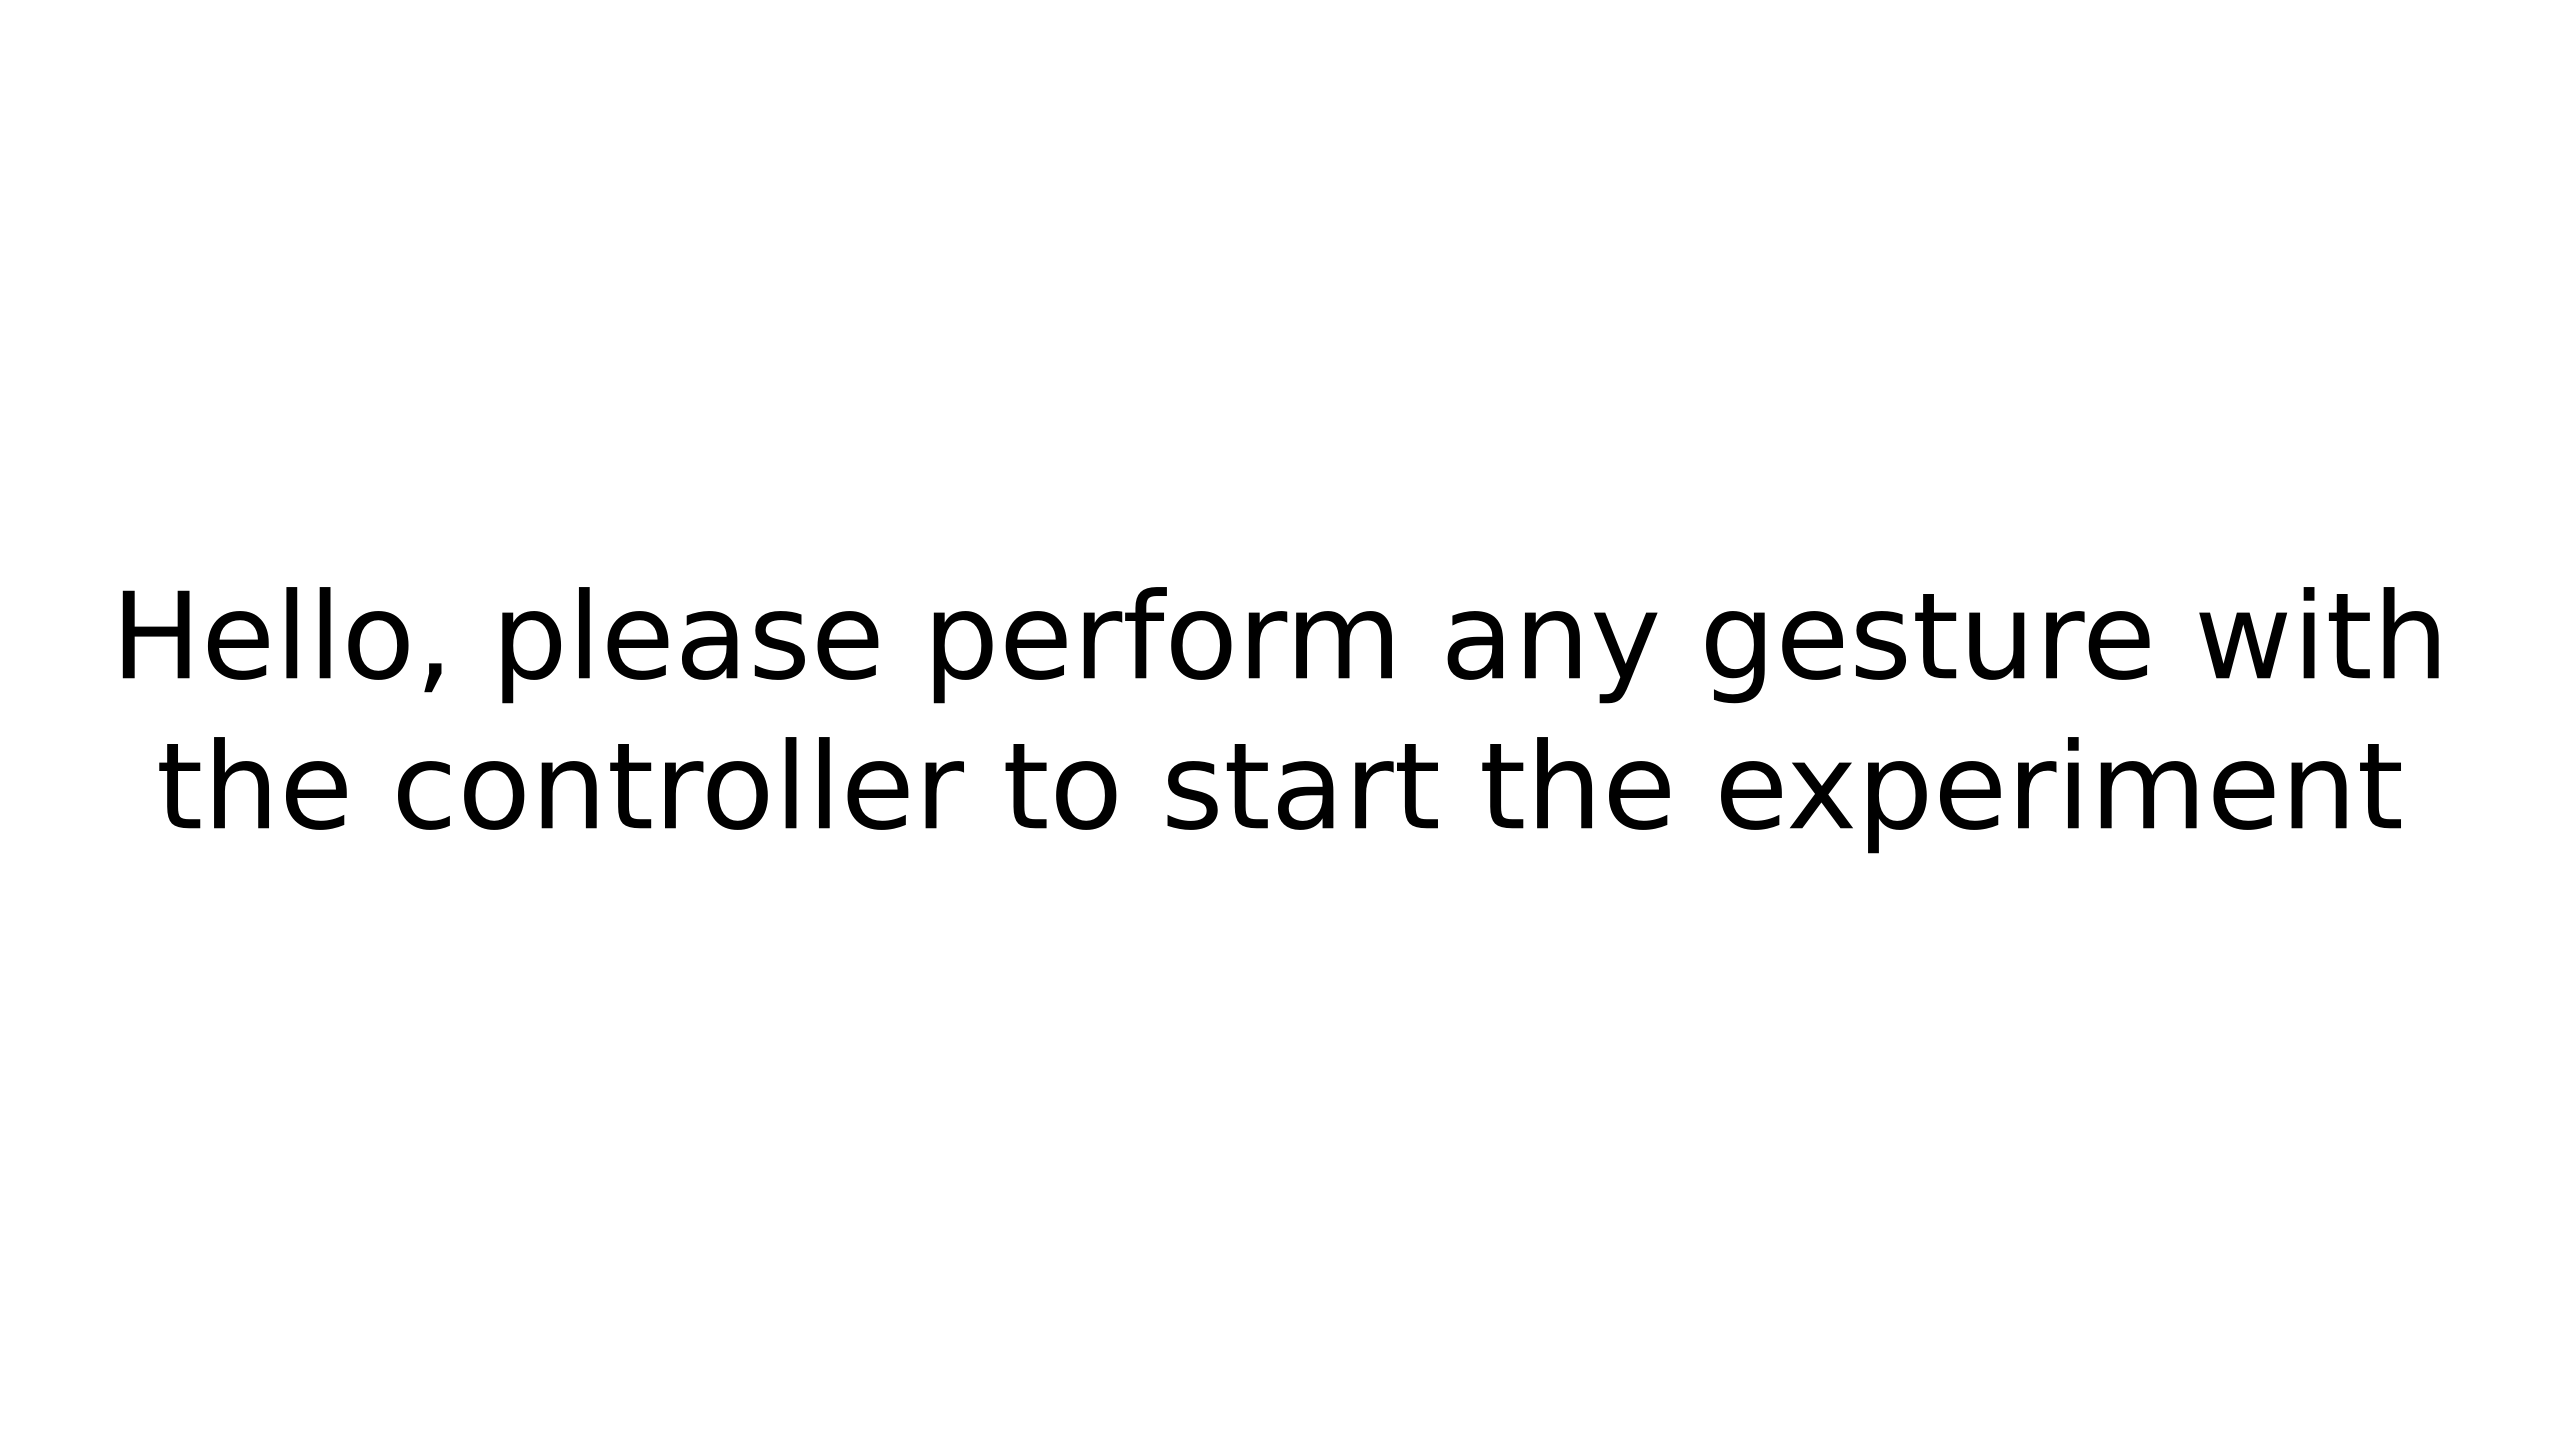
\includegraphics[width=0.24\textwidth]{1.png}} &
            \frame{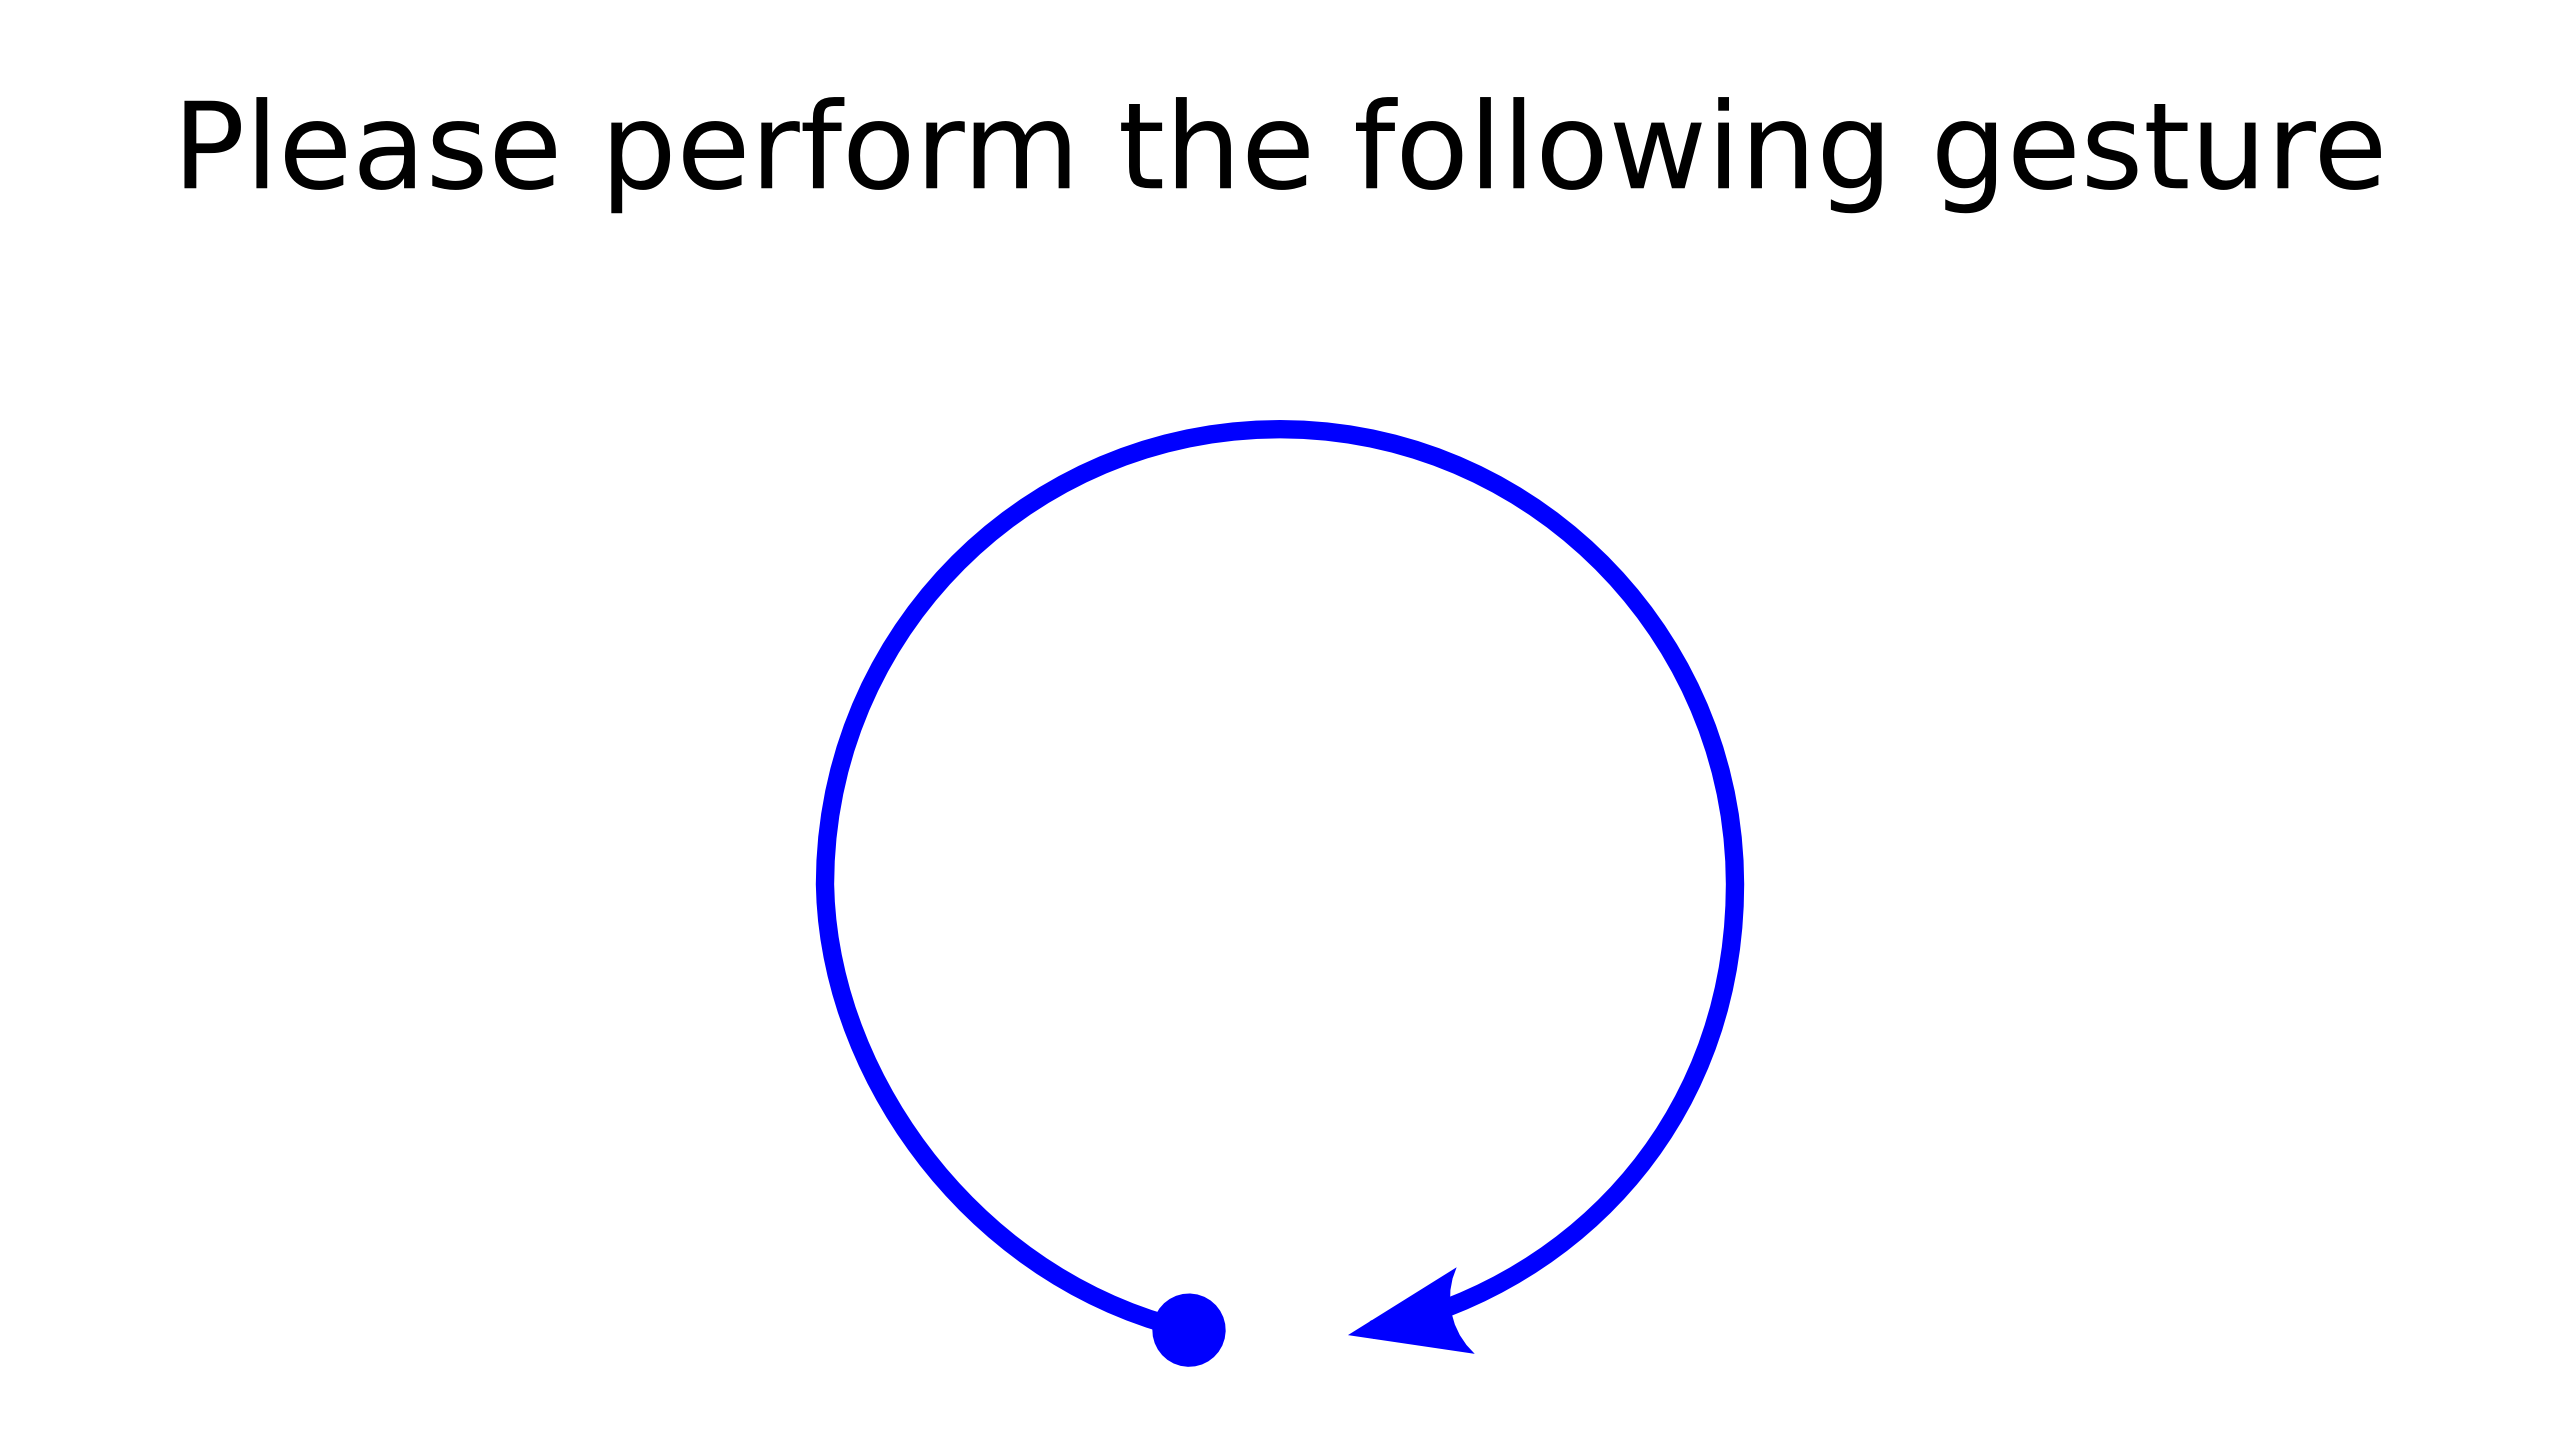
\includegraphics[width=0.24\textwidth]{2.png}} &
            \frame{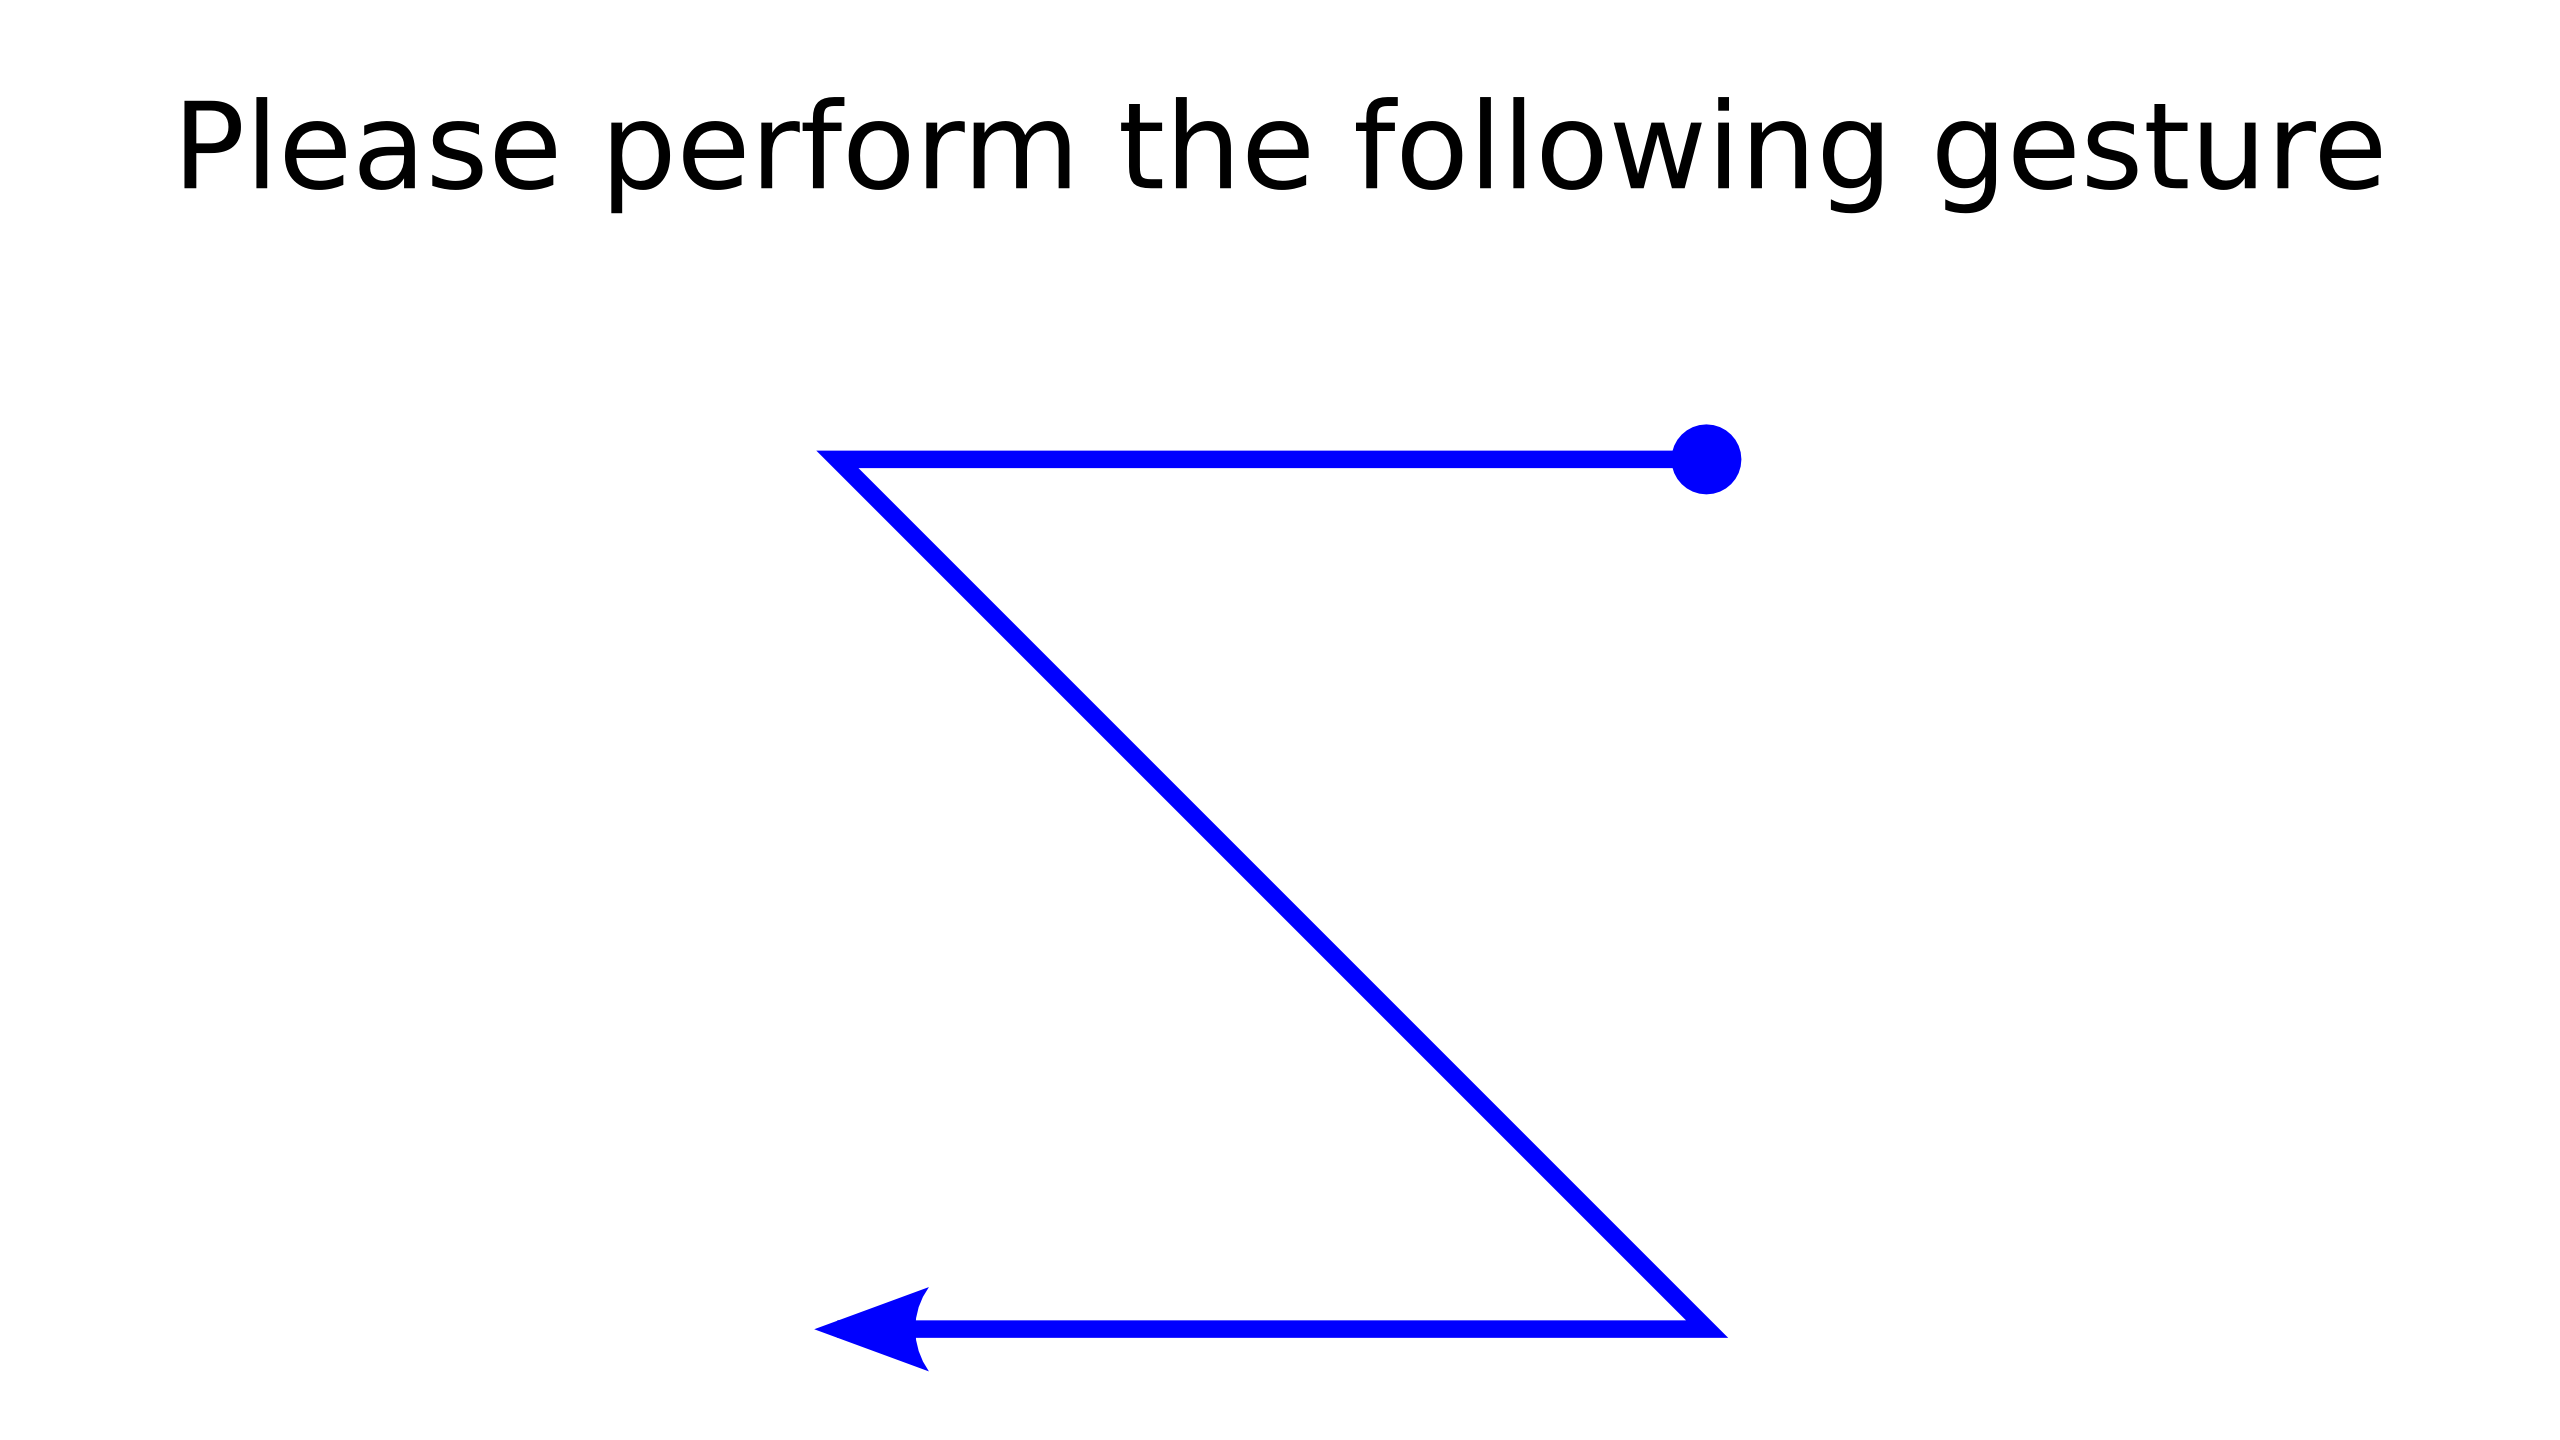
\includegraphics[width=0.24\textwidth]{3.png}} &
            \frame{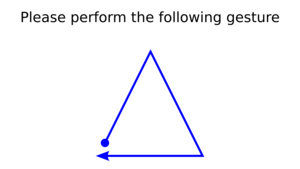
\includegraphics[width=0.24\textwidth]{4.png}} \\
            (a) \vspace{0.5ex} & (b) \vspace{0.5ex} & (c) \vspace{0.5ex} & (d) \vspace{0.5ex} \\
            \frame{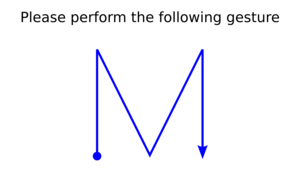
\includegraphics[width=0.24\textwidth]{5.png}} &
            \frame{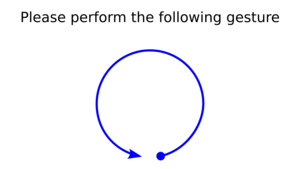
\includegraphics[width=0.24\textwidth]{6.png}} &
            \frame{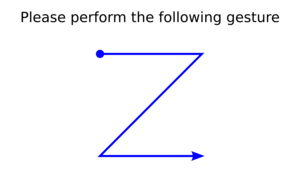
\includegraphics[width=0.24\textwidth]{7.png}} &
            \frame{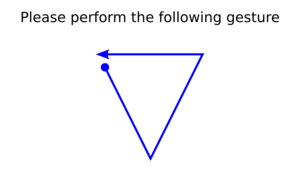
\includegraphics[width=0.24\textwidth]{8.png}} \\
            (e) \vspace{0.5ex} & (f) \vspace{0.5ex} & (g) \vspace{0.5ex} & (h) \vspace{0.5ex} \\
            \frame{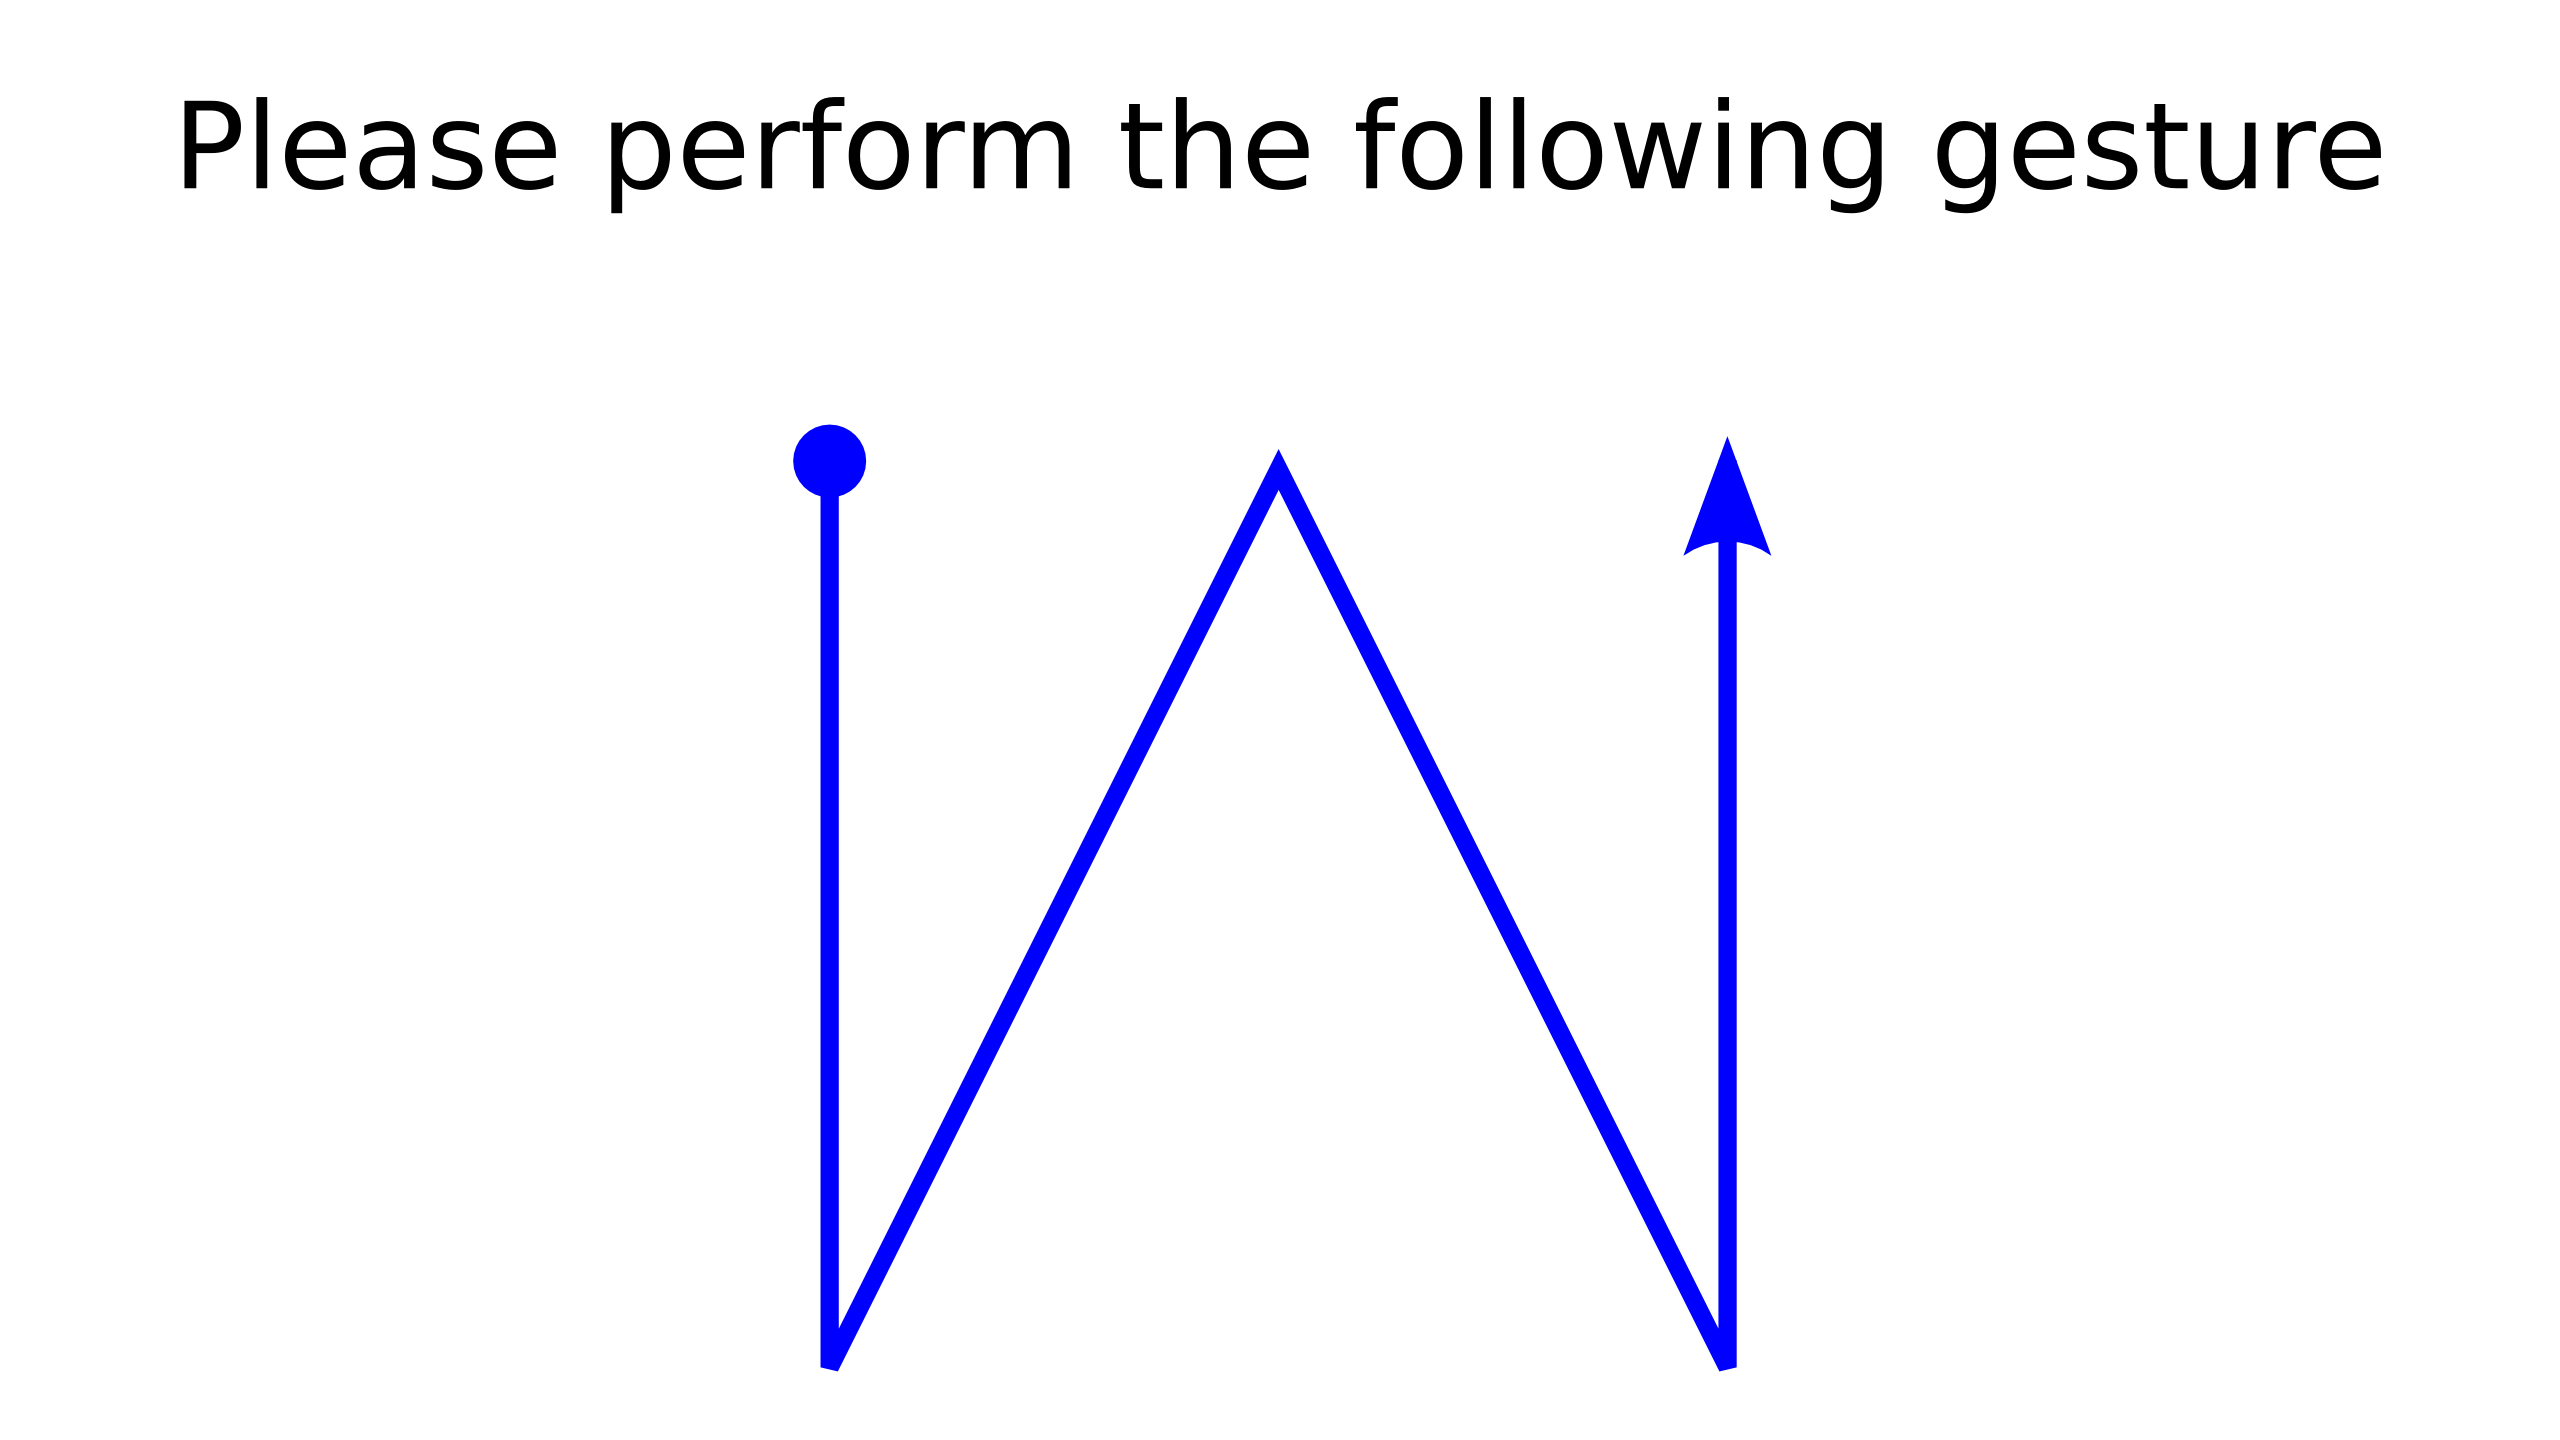
\includegraphics[width=0.24\textwidth]{9.png}} &
            \frame{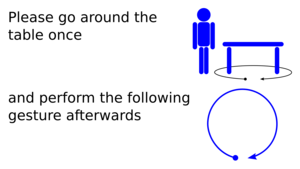
\includegraphics[width=0.24\textwidth]{10.png}} &
            \frame{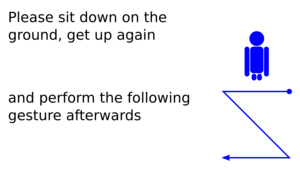
\includegraphics[width=0.24\textwidth]{11.png}} &
            \frame{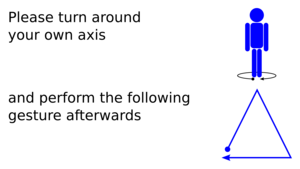
\includegraphics[width=0.24\textwidth]{12.png}} \\
            (i) \vspace{0.5ex} & (j) \vspace{0.5ex} & (k) \vspace{0.5ex} & (l) \vspace{0.5ex} \\
            \frame{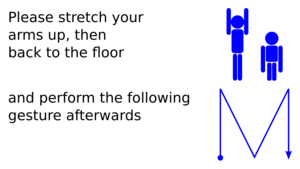
\includegraphics[width=0.24\textwidth]{13.png}} &
            \frame{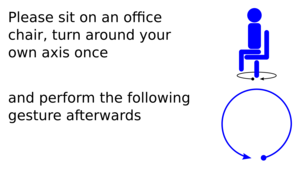
\includegraphics[width=0.24\textwidth]{14.png}} &
            \frame{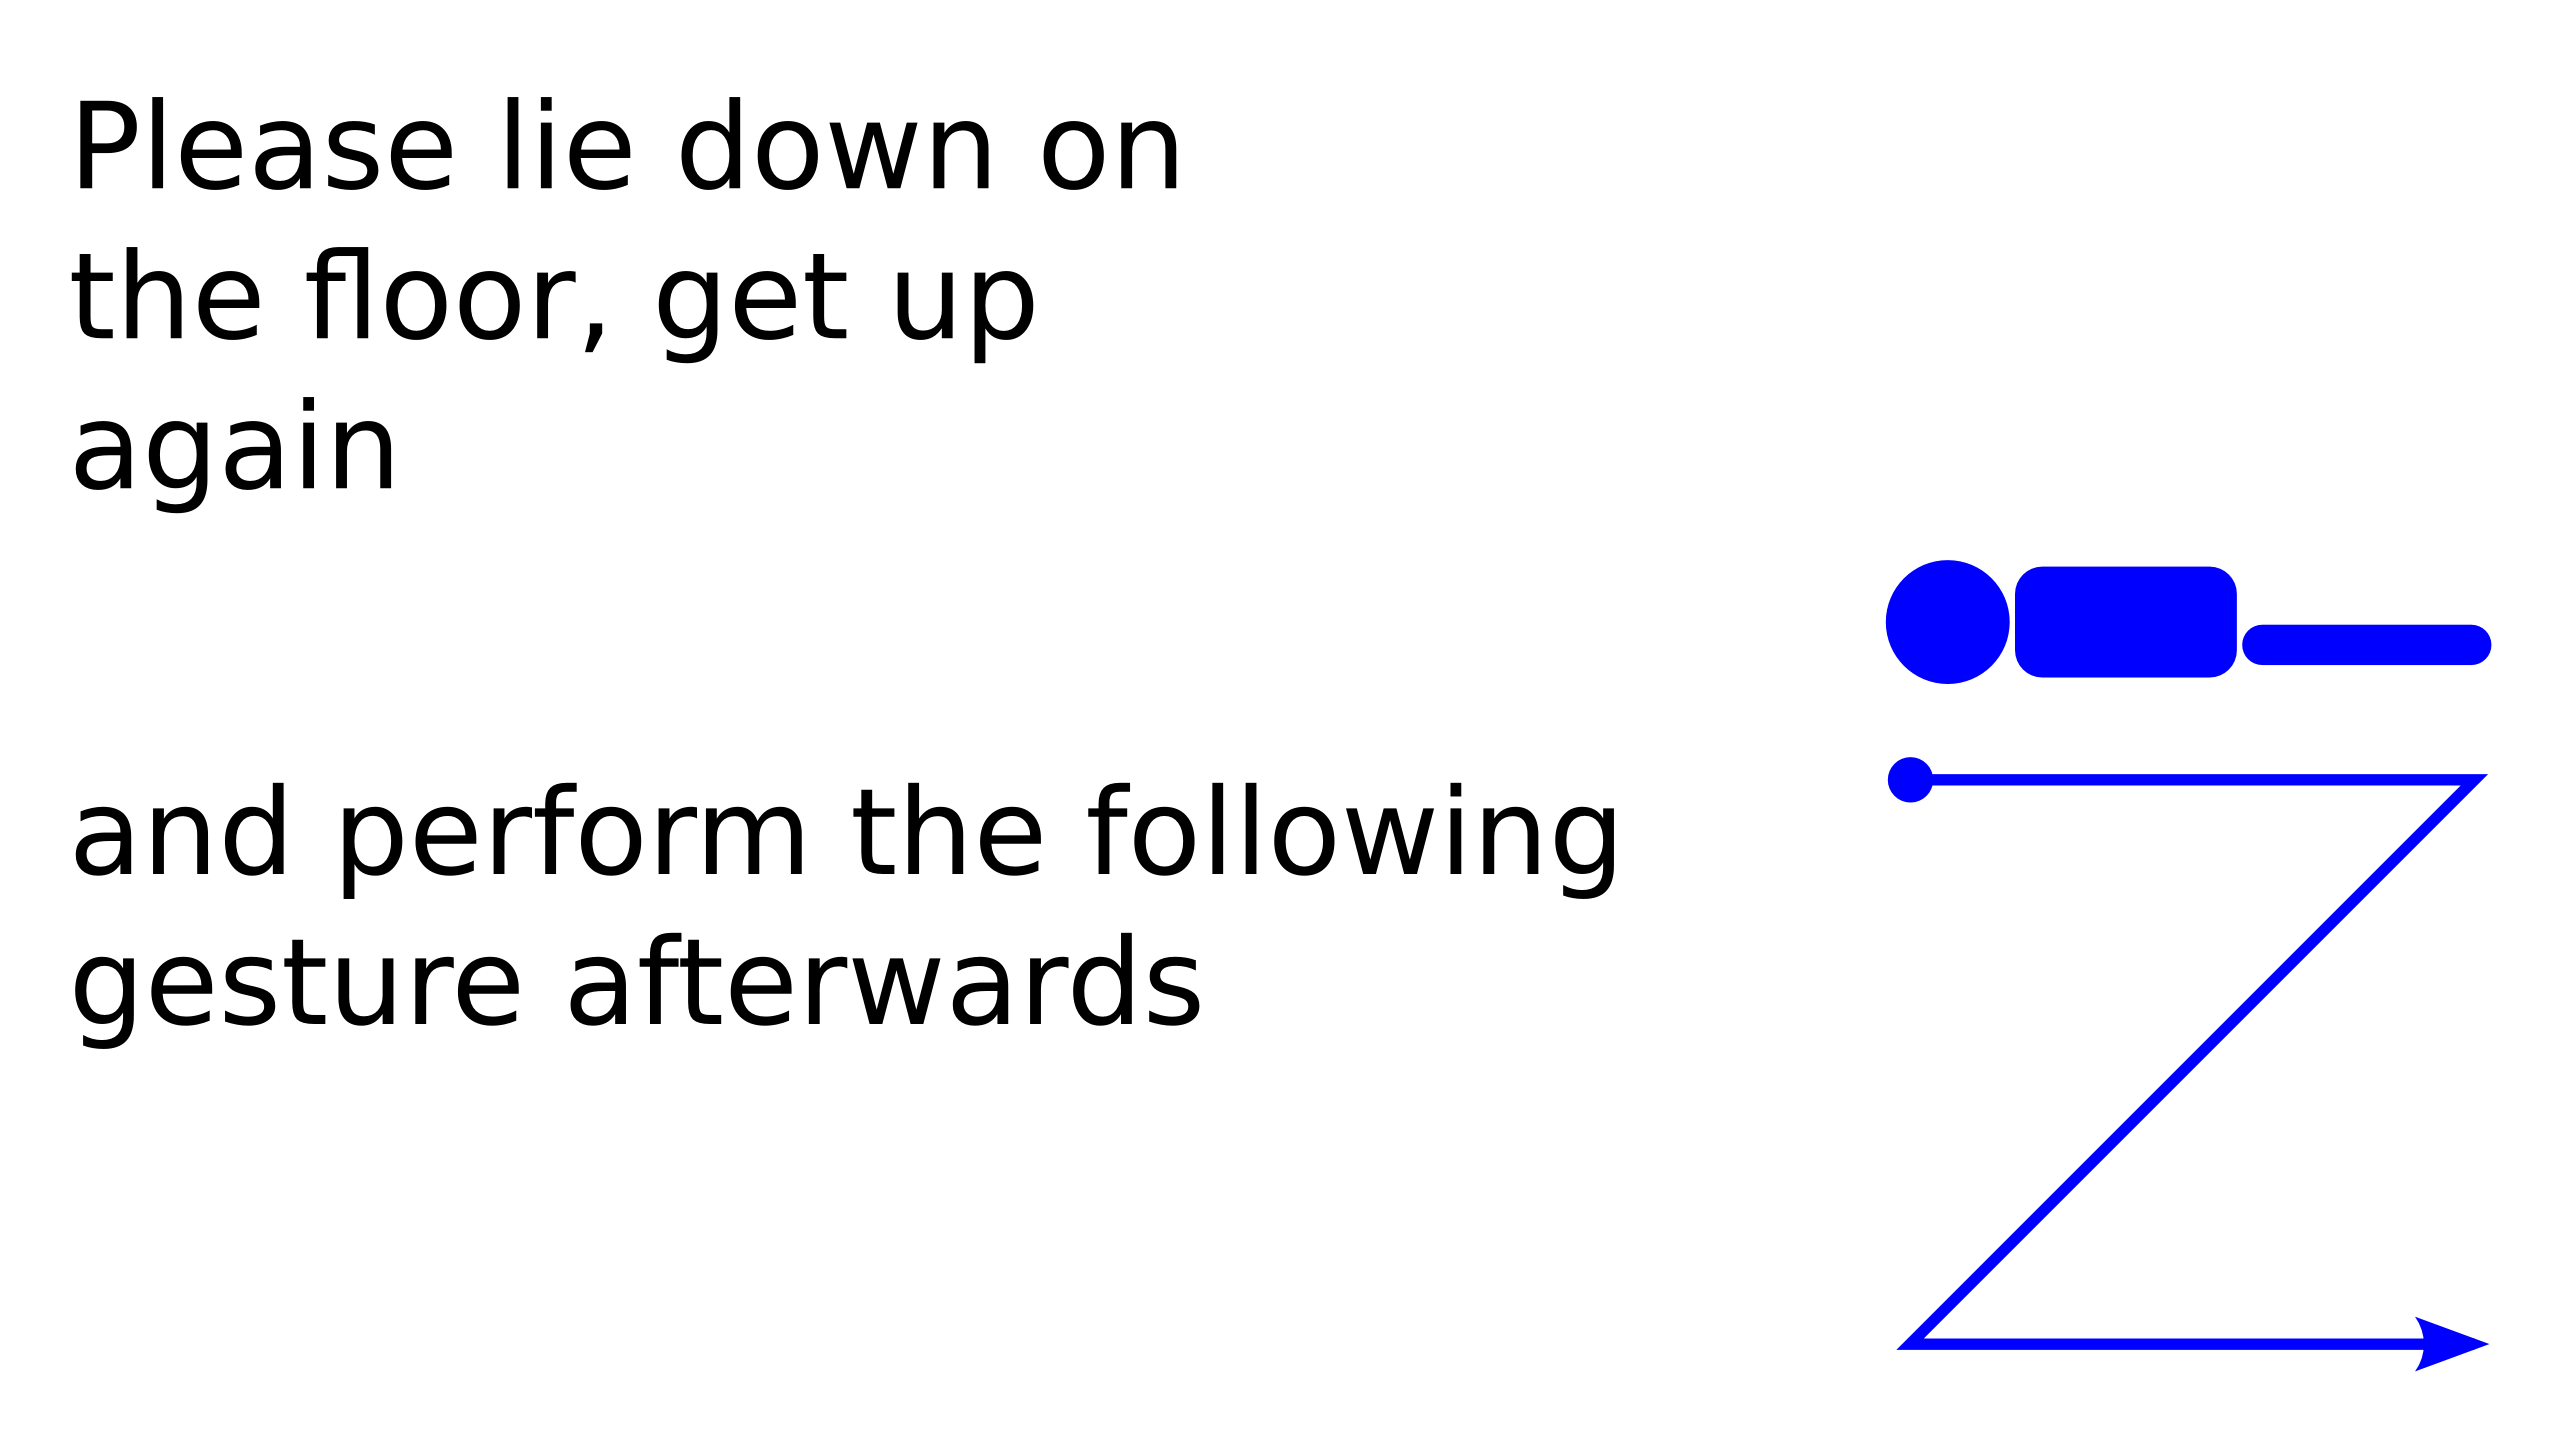
\includegraphics[width=0.24\textwidth]{15.png}} &
            \frame{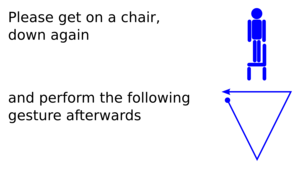
\includegraphics[width=0.24\textwidth]{16.png}} \\
            (m) \vspace{0.5ex} & (n) \vspace{0.5ex} & (o) \vspace{0.5ex} & (p) \vspace{0.5ex} \\
            \frame{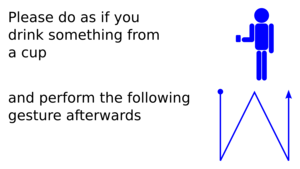
\includegraphics[width=0.24\textwidth]{17.png}} &
            \frame{
\includegraphics[width=0.24\textwidth]{18.png}} &
            \frame{
\includegraphics[width=0.24\textwidth]{19.png}} & \\
            (q) & (r) & (s) & \\
        \end{tabular}
    \end{center}
    \caption{The slides that are guiding the experimentees.}
    \label{fig:slides}
\end{figure}

Slide (a) of figure~\ref{fig:slides} has the task to welcome the experimentee and is later used in evaluation to mark
the start of the recording. 
